\chapter{Principes fondamentaux}

La thermodynamique est la description macroscopique des propriétés de la matière en termes de grandeurs physiques spécifiques et établissement de relations universelles entre ces grandeurs. Globalement, elle correspond à l'étude des phénomènes thermiques, liés à la dynamique du système étudié, c'est-à-dire les échanges et transferts d'énergie et de chaleur. Pour certains physiciens, la thermodynamique constitue aussi en la physique statistique, un domaine s'inquiétant plutôt du domaine microscopique, mais que nous n'étudierons pas ici.\\

Le principe donc, de cette étude à échelle macroscopique, se base sur l'étude de grandeurs exclusivement observables, comme le sont la pression, la température, le volume, ...\\

A partir de ces grandeurs, on est capable de rendre compte des échanges d'énergies mais, encore une fois, uniquement à l'échelle macroscopique. En effet, à l'échelle microscopique, il faudrait étudier mécaniquement nos systèmes, selon la mécanique de Newton, et, lorsque notre échelle d'étude est la mole, soit $6,022.10^{23}$ particules, on s'imagine difficilement effectuer le même nombre d'intégrales. A noter que la physique statistique s'intéresse à des échelles allant de $10^6$ à $1$ particules. \\

Quoiqu'il en soit, notre approche macroscopique nous ramène à des phénomènes observables à l'oeil nu, ou du moins, plus facilement visualisables, basés sur le comportement collectif des molécules et donc mesurables au cours d'une expérience. En effet, la thermodynamique est une science expérimentale, qui a permis de déterminer et de construire un socle théorique, qui a donné l'ensemble des lois générales que l'on étudiera en thermodynamique classique. \\

Dans ce premier chapitre, nous allons exclusivement nous focaliser sur les définitions et les principes fondamentaux de la thermodynamique, qui seront les prérequis nécessaires à la compréhension de l'ensemble des autres notions abordées par la suite ainsi que la compréhension des exercices.

\section{Vocabulaire thermodynamique}

Introduisons tout d'abord quelques définitions fondamentales au cadre de nos raisonnements thermodynamiques.

\subsection{Système et milieu expérimental}

Notre milieu expérimental est divisé en deux parties : le \textbf{système} que l'on note $\Sigma$, et l'extérieur. L'ensemble de ces deux parts de notre milieu expérimental forme l'univers. Parfois, entre ce système et l'extérieur, nous avons des frontières fictives mais aussi des frontières réelles. En réalité, ces frontières sont uniquement des productions de notre esprit, une volonté du thermodynamicien que vous êtes, de déterminer ces deux parties de l'univers, qui doivent idéalement être définies de façon à être cohérentes avec ce que nous cherchons à déterminer. Si on prend l'exemple de l'étude d'un moteur, dans une voiture, on comprend bien que l'étude thermodynamique se cantonnera strictement au moteur, mais si maintenant on s'intéresse à la détente adiabatique d'un cylindre d'un moteur, on se concentrera exclusivement sur ce cylindre et non l'ensemble du moteur.

\subsection{Principales grandeurs en thermodynamique}

Si bon nombre des grandeurs que nous définirons au cours de ces chapitres seront énoncés plus tard, il en est quelques unes qu'il est nécessaire de rapporter ici.\\

Introduisons maintenant une première grandeur : la quantité de chaleur, ou plus vulgairement \textbf{la chaleur}. La chaleur est une quantité d'énergie, elle est donc mesurée en joules (noté $J$, tel que $J = kg.m^2.s^{-2}$), et, elle correspond à l'énergie échangée sous forme de chaleur (ou agitation thermique) par un système, c'est-à-dire, l'énergie cédée ou reçue par notre système.\\

Une des autres grandeurs importantes est le \textbf{travail}, noté $W$, lui aussi est une énergie (donc mesuré en Joules), mais qui correspond plus, à de l'énergie sous la forme de l'application d'une force sur notre système ou un point précis de celui-ci, entraînant la déformation de notre système ou son déplacement.\\

La \textbf{pression}, est une composante importante de la thermodynamique, et correspond à l'effet de l'agitation des molécules sur une surface. de façon générale, elle correspond à une force appliquée sur une surface (soit $\overrightarrow{F}=P.d\overrightarrow{S}$). On la mesure en pascals (noté $Pa$, qu'on peut aussi exprimer en $N.m^{-2}$. De façon générale, la pression possède plusieurs unités, plus ou moins utilisées, comme :

\begin{itemize}
\item le bar, tel que $1~bar = 10^5 Pa$
\item l'atmosphère, noté $atm$ tel que $1~atm = 1,01325.10^5~Pa$
\item le millimètre de mercure, noté $mmHg$ tel que $1~mmHg=133,322~Pa$
\end{itemize}

La \textbf{température} est, elle aussi, une grandeur importante en thermodynamique, puisqu'elle rend compte de l'agitation thermique dans notre système. Mesurée dans le système international en Kelvin (noté $K$), on retrouve régulièrement des valeurs notées en degrés Celsius, plus facile à reconnaître, et basées sur la même échelle que le Kelvin, mais ne prenant pas la même origine. Ainsi, pour passer du degré Celsius au Kelvin, on ajoutera $273,15$, à notre valeur telle que : $0^{\circ}C=273,15~K$.\\

Pour finir, regardons rapidement la notion de \textbf{volume}, qui correspond à un espace en 3 dimensions occupé par de la matière. Attention, dans toute équation thermodynamique, le volume doit être en $m^3$ et non en litres, cette dernière unité n'étant pas une unité du système international.

\subsection{Variables, fonctions et équations d'état}

Les variables sont les grandeurs physiques permettant de décrire des phénomènes à l'échelle macroscopique comme la pression, la température, ... Une variable est dite \textbf{variable d'état} si on peut la mesurer uniquement indépendamment de son histoire thermodynamique. Si l'on définit une variable d'état en fonction d'autres variables d'état, on créé ainsi une fonction d'état. Une équation d'état, à partir d'une variable d'état donne toujours 0, telle que $f(X_1)=0$.\\

Si nous détaillons plus les variables, nous pouvons les classer telles que : une variable peut être extensive ou intensive, ainsi que externe et interne. \\

Une variable \textbf{extensive} est une variable qui possède des propriétés d'additivité comme la masse ou le volume. A l'inverse, une variable est \textbf{intensive} si celle-ci n'est pas additive et est donc indépendante de la masse, comme c'est le cas de la pression, la température.\\

D'autre part, une variable est dite \textbf{externe} si elle imposée et contrôlée par l'extérieur. A contrario, une variable sera \textbf{interne}, si celle-ci est scrupuleusement liée au système, et permet de décrire son équilibre thermodynamique.

\subsection{États de la matière}

Pour conclure sur ces quelques définitions, détaillons les différents états de la matière, socle de notre connaissance physique et chimique de notre monde, mais dont la définition n'est pas toujours aisée : 
\begin{itemize}
\item \textbf{État gaz} : état peu dense (ou dilué), dont les particules subissent peu d'interactions, et sont désordonnées.
\item \textbf{État liquide }: état dense, dont les particules subissent des interactions non négligeables, et sont ordonnées à courte portée, mais désordonnées à longue portée.
\item \textbf{État solide }: état très dense, où les particules subissent des interactions fortes, et sont ordonnées à tous les niveaux.
\end{itemize}

\section{Systèmes et transformations}

Avant de détailler les différents types de systèmes et les transformations que ceux-ci peuvent subir, introduisons la convention de signe que l'on utilise en thermodynamique : lorsqu'un système reçoit de l'énergie notée $E$, on aura $\Delta E > 0$ ; et lorsqu'un système cède de l'énergie, on aura $\Delta E < 0$.

\subsection{Types de systèmes}

La caractérisation d'un système peut permettre de déterminer parfois, bon nombre de valeurs, avant même d'avoir commencé à étudier les réactions thermodynamiques.\\

\pagebreak 

Synthétiquement, on a :

\begin{figure}[H]
\centering
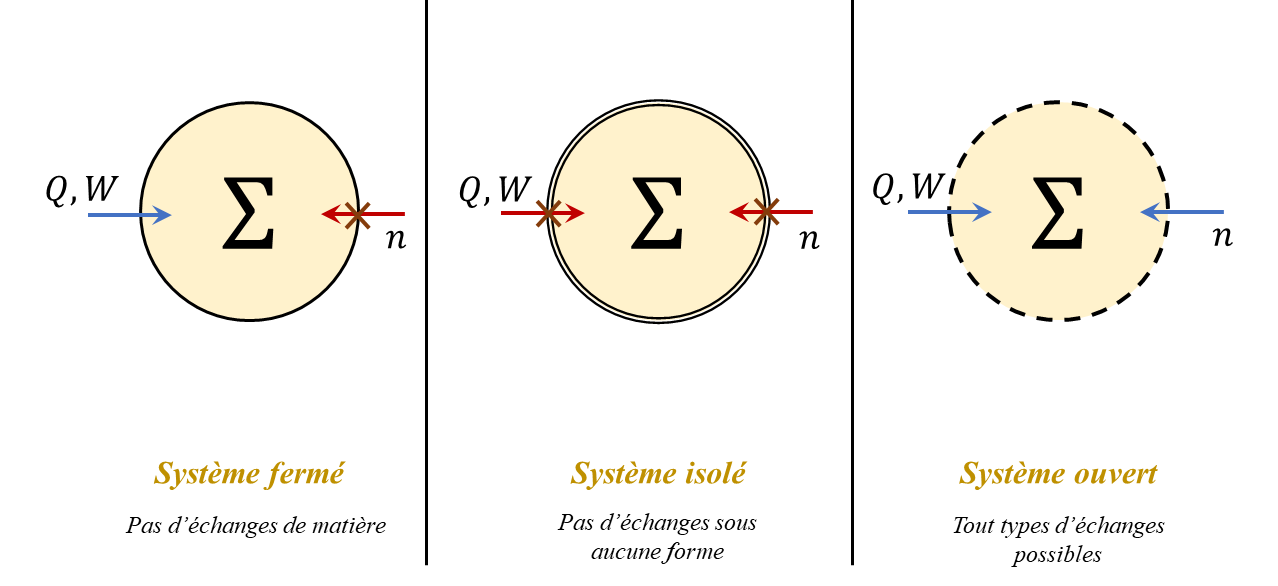
\includegraphics[scale=0.35]{Diapositiv2.PNG}
\caption{Cas de plusieurs systèmes thermodynamiques}
\end{figure}

Si on détaille un peu, on a d'une part un système \textbf{fermé}, qui n'échange pas de matière, mais permet le passage de l'énergie. D'autre part, on a deux autres systèmes totalement opposés que sont le système \textbf{isolé}, qui n'échange rien, et le système \textbf{ouvert} qui lui, permet l'échange de chaleur et de matière.

\subsection{Transformations}

Une transformation est une perturbation de l'état d'équilibre, qui peut correspondre à la variation d'une variable, ou la supression d'une contrainte. La caractérisation d'une transformation thermodynamique correspond au passage d'un état initial à un état final. Schématiquement, on a :
$$ \begin{array}{ccc}E_{initial}& \longrightarrow& E_{final}\\X_i,Y_i,Z_i, ...&&X_f, Y_f, Z_f, ...\end{array}$$
Quand on a un état initial égal, à l'état final, on dit qu'on a un \textbf{cycle thermodynamique}. Au cours d'un cycle thermodynamique, un système va subir plusieurs transformations, celles-ci pouvant être réversibles ou non, mais aussi quasi-statiques.\\

\begin{figure}[h!]
\centering
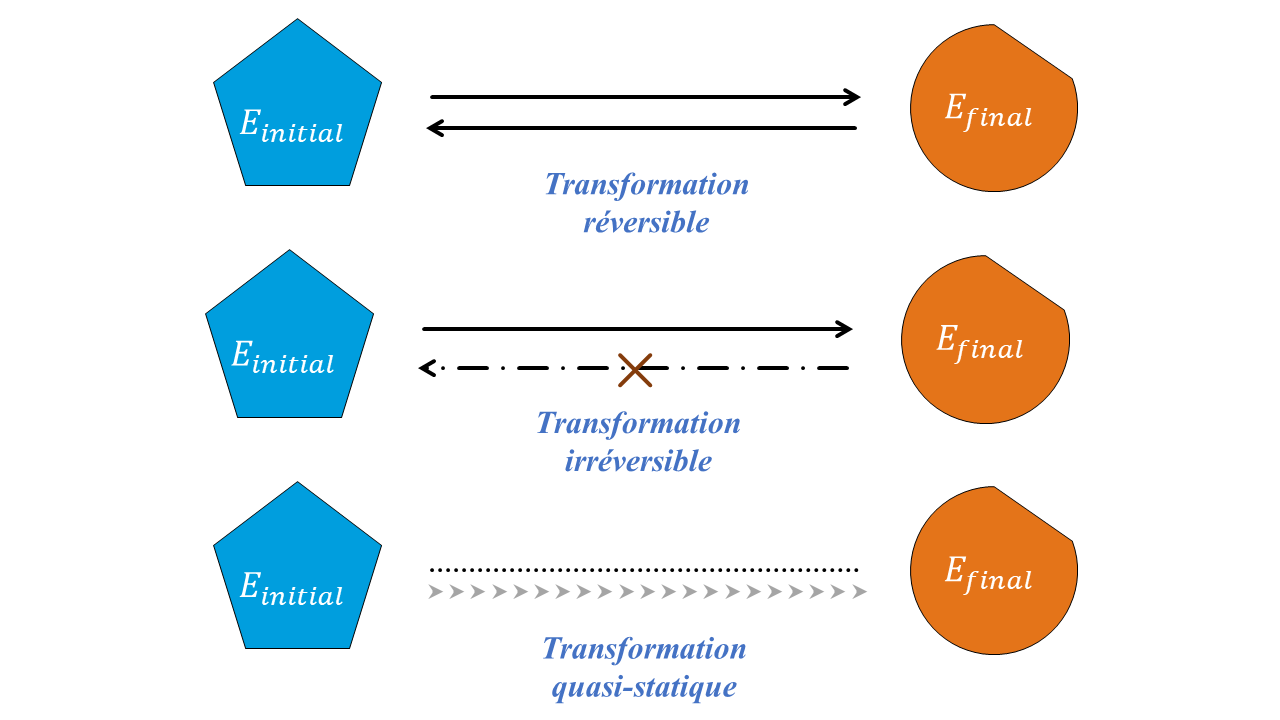
\includegraphics[scale=0.3]{Diapositiv3.PNG}
\caption{Transformations et leurs caractéristiques}
\end{figure}

Une transformation est dite \textbf{réversible} si , il est possible, en faisant la transformation inverse, de retourner à l'état initial. Cette transformation est possible du fait qu'elle soit composée de successions de micro-états d'équilibres.\\

Une transformation est dite, a contrario, \textbf{irréversible}, s'il n'est pas possible de revenir à l'état initial, conséquence, expliquée par l'inexistence de micro-états d'équilibres.\\

Pour finir, il existe des transformations \textbf{quasi-statiques}, qui sont caractérisées par des états d'équilibres lents, associés à une transformation très lente voire quasi-statique. C'est le cas des réactions réversibles \footnote{Attention ! La réciproque n'est pas vrai : il existe de nombreuses réactions irréversibles quasi-statiques}.\\

Au delà de ce cadre, il existe des transformations bien spécifiques, où les conditions d'évolution sont bien déterminées, ce qui nous permet d'en déduire de nombreuses informations sur les évolutions de nos variables au sein de notre système :

\begin{itemize}
\item Une transformation \textbf{monotherme}, est une transformation pour laquelle la température initiale sera égale à la température finale.
\item Une transformation \textbf{isotherme}, est une transformation ou la température est une constante tout au long de l'expérience.
\item Une transformation \textbf{isochore}, est un transformation pour laquelle, le volume est constant.
\item Une transformation \textbf{ isobare}, est une transformation pour laquelle la pression reste constante au cours de la transformation.
\item Une transformation \textbf{adiabatique}, est une transformation au cours de laquelle, aucun échanges de chaleur ne sera possible, soit $Q=0$.
\end{itemize}

Si on résume schématiquement l'ensemble de ces transformations spécifiques, on obtient :

\begin{figure}[h!]
\centering
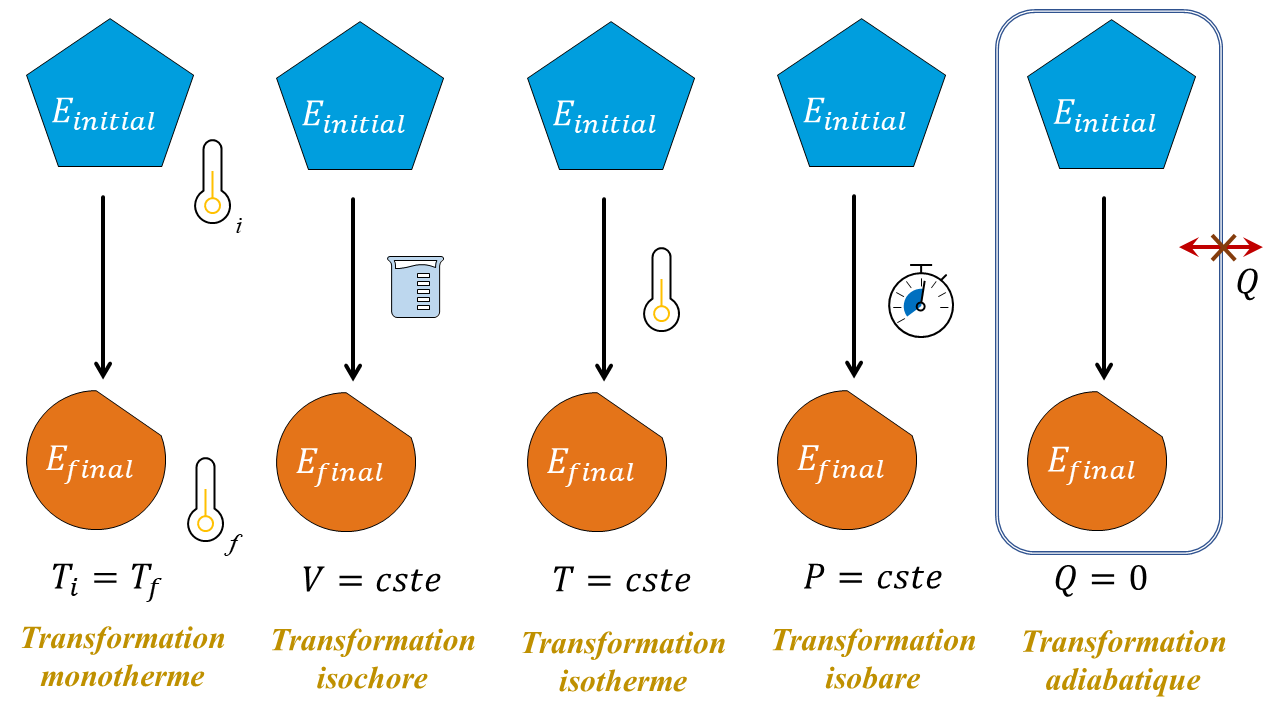
\includegraphics[scale=0.35]{Diapositiv4.PNG}
\caption{Transformations spécifiques d'un système thermodynamique}
\end{figure}

Si on se focalise maintenant exclusivement sur les échanges de chaleur, que l'on évalue selon $Q$, on décrit une transformation \textbf{endothermique}, telle une transformation pour laquelle notre système gagne de la chaleur ; une transformation \textbf{exothermique} qui, a l'inverse, correspond à la perte de chaleur par notre système ; et pour finir, une transformation \textbf{athermique}, pour laquelle il n'y a pas d'échanges de chaleur avec le milieu extérieur à notre système. \\



Si on représente cela schématiquement, on obtient :

\begin{figure}[h!]
\centering
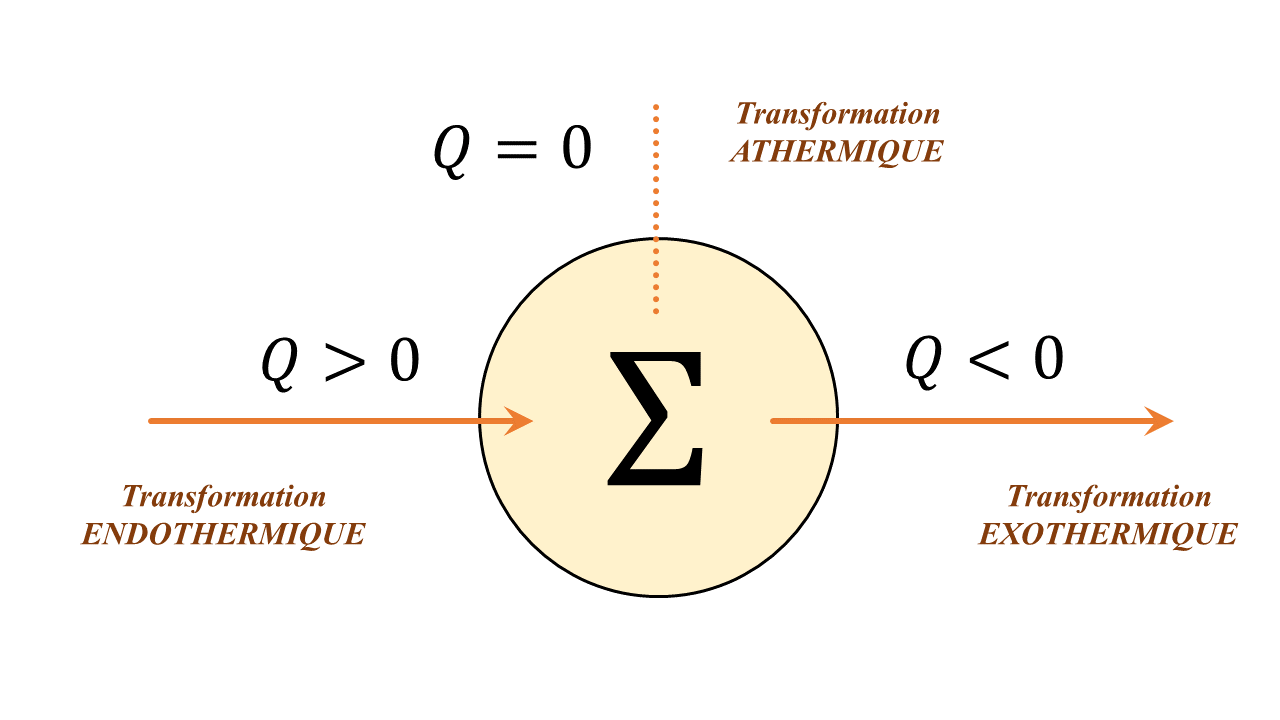
\includegraphics[scale=0.4]{Diapositiv1.PNG}
\caption{Échange de chaleur par un système au cours d'une transformation}
\end{figure}

A noter que, si une paroi est adiabatique, cela veut dire qu'elle ne permet aucun échanges de chaleur, mais que si la paroi d'un système est \textbf{diatherme}, alors celle-ci laisse passer la chaleur.

\subsection{Transformations chimiques}

Une transformation, ou réaction chimique, est caractérisée par la rupture et la formation de liaisons covalentes (liaisons allant de $0,9 \angstrom$ à $1,3\angstrom$). Dans ce cas, l'état initial correspond aux réactifs, et l'état final aux produits.

$$aA+bB \rightleftharpoons cC + dD$$

L'avancement de la réaction, noté $\xi$ est alors définit tel que :
$$\xi = \frac{n(A)-n_0(A)}{a}=\frac{n(B)-n_0(B)}{B}=\frac{n(C)-n_0(C)}{c}=\frac{n(D)-n_0(D)}{d}$$

On peut ainsi définir le taux d'avancement $\Gamma$ d'une réaction exprimé tel que :
$$\Gamma =\frac{n_{i,0}-n_{\xi}}{n_{i,0}}$$
